\chapter{Networks with costs, respectively upper/lower bounds}

\section{Networks with costs}\index{Networks with costs}

Get rid of parallel and antiparallel edges, cost: $E \rightarrow \mathbb{R}$ 

\begin{example}
\underline{case a)}\\

\begin{figure}[h]
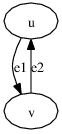
\includegraphics[scale=0.45]{diagrams/graph5_1}
\caption{With antiparallel edges}
\label{G1}
\end{figure}

\begin{figure}[h]
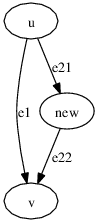
\includegraphics[scale=0.45]{diagrams/graph5_2}
\caption{With antiparallel edges}
\label{G2}
\end{figure}

\ref{G1} is transformed to \ref{G2}
\\
$c(e{_1})$ as before $c$.\\
$cost(e{_21}) = cost(e{_2})$\\
$cost(e{_22}) = 0$\\
$cost(e{_21}) = cost(e{_22}) = cost(e{_2})$\\

\underline{case b)}\\

\begin{figure}[h]
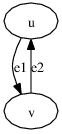
\includegraphics[scale=0.45]{diagrams/graph5_1}
\caption{With antiparallel edges}
\label{fig:G3}
\end{figure}

\begin{figure}[h]
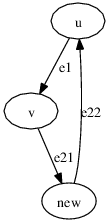
\includegraphics[scale=0.45]{diagrams/graph5_3}
\caption{After transformation - without antiparallel edges}
\label{fig:G4}
\end{figure}

\ref{fig:G3} is transformed to \ref{fig:G4}\\
\end{example}

From now on we consider only networks without parallel/antiparallel edges.

\begin{definition}
Let $G=(V,E)$ with $s, t \in V, c: E \rightarrow \mathbb{R^+}$ be a network. Let cost: $E \rightarrow \mathbb{R}$ be a function that associates ``cost'' to every edge.
Let f be a flow function for this network. \\

$cost(f) = \sum\limits_{e \in E} f(e) * cost(e)$\\

\end{definition}


\textbf{Task:}\\
Given:
\begin{enumerate}
  \item a network $G=(V,E), s, t \in V, c, cost$
  \item $w \in \mathbb{R^+}$
\end{enumerate}
Find a flow function f with total flow $F=w$ and minimal costs.


\begin{definition}
$G=(V,E), s, t \in V, c, cost, f flowfunction$\\
The graph $G{_f}=(V,E{_f})$ with $\tilde{c}$, $\tilde{costs}$.\\
Let $e=(u,v) \in E$
\begin{enumerate}
  \item If $f(e) < c(e)$ then $e{_1}=(u,v) \in E{_f}$\\
  $\tilde{c}(e{_1}) = c(e) - f(e) > 0 $\\
  $\tilde{cost}(e{_1}) =  cost(e)$\\
  \item If 0 < $f(e)$ then $e{_2}=(v,u) \in E{_f}$\\
   $\tilde{c}(e{_2}) = f(e)$\\
   $\tilde{cost}(e{_2}) =  - cost(e)$\\
\end{enumerate}
\end{definition}

\textbf{Observation:}\\
\begin{enumerate}[label=\alph*]
  \item 
  If $e \in E$ is an edge with $0 < f(e) < c(e)$\\
\begin{figure}[h]
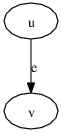
\includegraphics[scale=0.45]{diagrams/graph5_4}
\caption{$G=(V,E)$}
\label{fig:G5}
\end{figure}  
\begin{figure}[h]
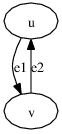
\includegraphics[scale=0.45]{diagrams/graph5_1}
\caption{$G{_f}$}
\label{fig:G6}
\end{figure}    

\item 
If $e \in E$ is an edge with $0 < f(e) = c(e)$ - as shown in \ref{fig:G7}.
\begin{figure}[h]
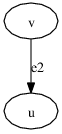
\includegraphics[scale=0.45]{diagrams/graph5_5}
\caption{$G{_f}$}
\label{fig:G7}
\end{figure}

\item
If $e \in E$ is an edge with $0 = f(e) < c(e)$ - as shown in \ref{fig:G8}.
\begin{figure}[h]
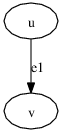
\includegraphics[scale=0.45]{diagrams/graph5_6}
\caption{$G{_f}$}
\label{fig:G8}
\end{figure}

\item 
If $e \in E$ is an edge with $0 = f(0) = c(0)$ - as shown in \ref{fig:G9}.
\begin{figure}[h]
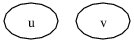
\includegraphics[scale=0.45]{diagrams/graph5_7}
\caption{$G{_f}$}
\label{fig:G9}
\end{figure}
\end{enumerate}

\begin{definition}
Let p be a directed cycle in $G{_f}$.
$cost (p) := \sum\limits_{e \in P} cost(e)$
\end{definition}

\begin{example}

\begin{figure}[h]
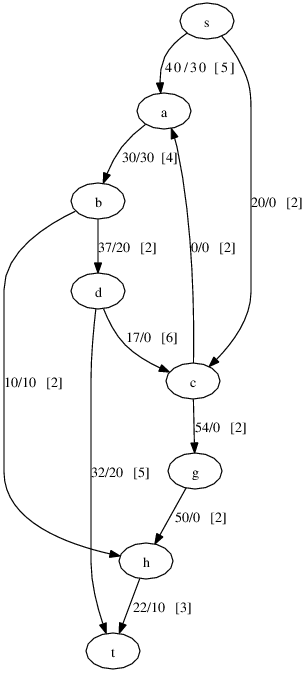
\includegraphics[scale=0.45]{diagrams/graph5_8}
\caption{$G$}
\label{fig:G10}
\end{figure}

\begin{figure}[h]
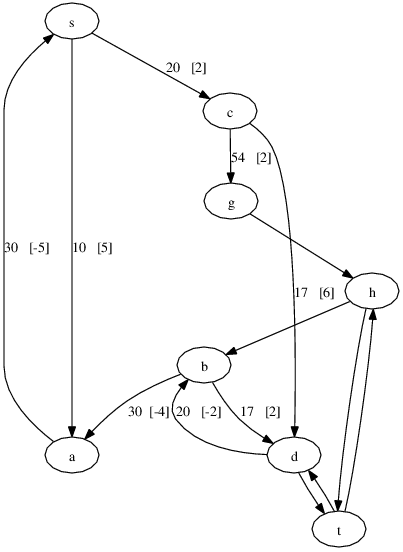
\includegraphics[scale=0.45]{diagrams/graph5_9}
\caption{$G{_f}$}
\label{fig:G11}
\end{figure}

directed cycles of negative costs:
$t - h - b - d - t \rightarrow -1$\\
$s - c - g - h- b - a - s \rightarrow -5$\\
\end{example}


\textbf{Theorem 5.1}\\
Let a network with cost function be given and a flow function f with total flow $F=w$. $f$ has least costs among all flow functions with total flow $w$ if and only if $G{_f}$ does not have any directed cycles of negative cost.

\begin{proof}
``$\implies$'' Let f be a cost minimal flow function with total flow $F=w$. Assume that $G{_f}$ contains a directed cycle of negative costs. Adapting the flow values along this cycle in the original network we can reduce the cost while maintaining the total flow.
\end{proof}

\begin{example}

\begin{figure}[h]
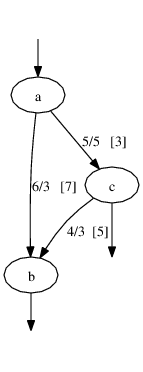
\includegraphics[scale=0.5]{diagrams/graph5_10}
\caption{$G{_f}$}
\label{fig:G12}
\end{figure}

\begin{figure}[h]
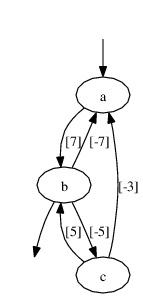
\includegraphics[scale=0.5]{diagrams/graph5_11}
\caption{$G{_f}$}
\label{fig:G13}
\end{figure}


For edges that correspond to forward edges (of type $e{_1}$) we may raise the flow value.
For edges that correspond to backward edges (of type $e{_1}$) we may reduce the flow.

\end{example}



\begin{lemma}
Let f be  flow function with total flow $F=w$ and let f be cost minimal. Let p be an augmenting path that is cost minimal then the resulting flow f' constructed from f and p is cost minimal for $w+\Delta$ ($\Delta$ from the augmenting path).
\end{lemma}

\section{Networks with upper and lower bounds}

we associate with each edge e a lower bound $b(e)$ and request for the flow function additionally that:\\
$b(e) <= f(e)$\\
A flow function obeying this additional constraint is called \underline{legal flow function} (see \ref{fig:no_legal_flow}).

\begin{example}
\begin{figure}[t]
\centering
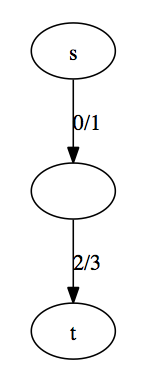
\includegraphics[scale=0.4]{diagrams/chapter_5_2_no_legal.png}
\caption{No legal flow possible for b(e)/c(e)}
\label{fig:no_legal_flow}
\end{figure}
\end{example}

To answer the question if there is a legal flow for a network with lower/upper bounds we proceed on follows. Construct the Graph $\Bar{G} = (\Bar{V},\Bar{E})$.

\begin{enumerate}
  \item $\Bar{V} = V \cup \{\Bar{s}, \Bar{t}\}$
  \item for every node $v \in V$ introduce an edge e from v to $\Bar{t}$.\\
  $\Bar{c}(e) = \sum\limits_{e \in \beta (v)} b(e)$\\
  $\Bar{b}(e) = 0$
  \item for every node $v \in V$ introduce an edge e from $\Bar{s}$ to v.\\
  $\Bar{c}(e) = \sum\limits_{e \in \alpha (v)} b(e)$\\
  $\Bar{b}(e) = 0$
  \item The edges in E remain but with new bunds:\\
  $\Bar{c}(e) = c(e) - b(e)$\\
  $\Bar{b}(e) = 0$
  \item Introduce edges from $s \overset{e}\rightarrow t$, $t \overset{e'}\rightarrow s$ with:\\
  $\Bar{c}(e) = \Bar{c}(e') = \infty$\\
  $\Bar{b}(e) = \Bar{b}(e') = 0$
\end{enumerate}

Bar{E} consists of the edges in E plus the newly introduced edges.


\begin{lemma}
The original network with upper and lower bounds has a legal flow if and only if the maximum flow of the auiliary network saturates all edges emanating from $\Bar{s}$.
\end{lemma}


\textbf{Hint:}\\
Let $Bar{f}$ be a flow function for the associated network with maximal total flow then $f(e) = Bar{f}(e) + b(e)$ is a legal flow function ($e \in E$).

